\chapter{Комплексная оценка производительности ВС}

В настоящий момент списки Top50 и Top500
выстроены в порядке убывания пиковой производительности и производительности на тесте LinPack что, разумеется, дает определенную информацию
о сравнительной скорости работы представленных там машин. Но очень многие факторы, такие как скорость работы и объем дисков, пропускная 
способность шины памяти и коммуникационной сети, неоднородность оборудования и т.д. - остаются за пределами рассмотрения. А это именно те 
проблемы, с которыми придется столкнуться при попытке посчитать на кластере большую задачу. По этой причине тестирование продится с помью измерения времени, затрачитваемого на различные этапы программы, решающей реальную физическую задачу.

В \textbf{третьей главе} описана методика измерения характеристик ВС с помощью программы, релизующей метод частиц в ячейках.


\textbf{везде написать пиковые знач. - Курносов 
}


Предложена методика комплексной оценки тестируемой ВС с точки зрения возможности эффективной реализзации математических моделей на основе определения баланса между скоростью счета и скоростью пересылки данных между узлами ВС. Баланс определяется на основе усреднения данных расчетов по методу частиц в ячейках, который используется в качестве оценки снизу по скорости счета и оценки сверху по памяти для большинства существующих математических методов.

Кроме того, на основе проведенных расчетов измерена скорость счета и скорость перемещения данных для нескольких протестированных ВС.   

		
\textbf{сделать общий список всех расчетов, упоминающихся в..., для каждого укказать флопсы, в сравнениии с пиком, место в топ50 (с обясненнеим, почему наше лучше), для кого можно, производительность сети и общую оценку}

\textbf{Таблицу прогнозовов составляйт не только для гибридных, но и для всех, кого можно}



\section{Расчет производительности процессорных элементов}
\label{calc_PE}
В \textit{первом разделе} описана методика измерения производительности процессорных элементов.
Для того, чтобы отделить время счета от времени обращения к оперативной памяти было рассмотрено время работы процедуры,
реализующей одномерное преобразование Фурье, которая является частью физической диагностики, используемой в при моделировании динамики плазмы. Измереннное время с учетом известного размера данных и и количества операций в БПФ (\textit{Е.П.Овсянников и др.}), переводится во флопсы. Сравнительная производительность процессорных элементов некоторых из рассмотренных в диссертационной работе ВС выглядит как показано на рисунке  \ref{procs_flops}:

\begin{figure}[htb]
	\begin{center}
		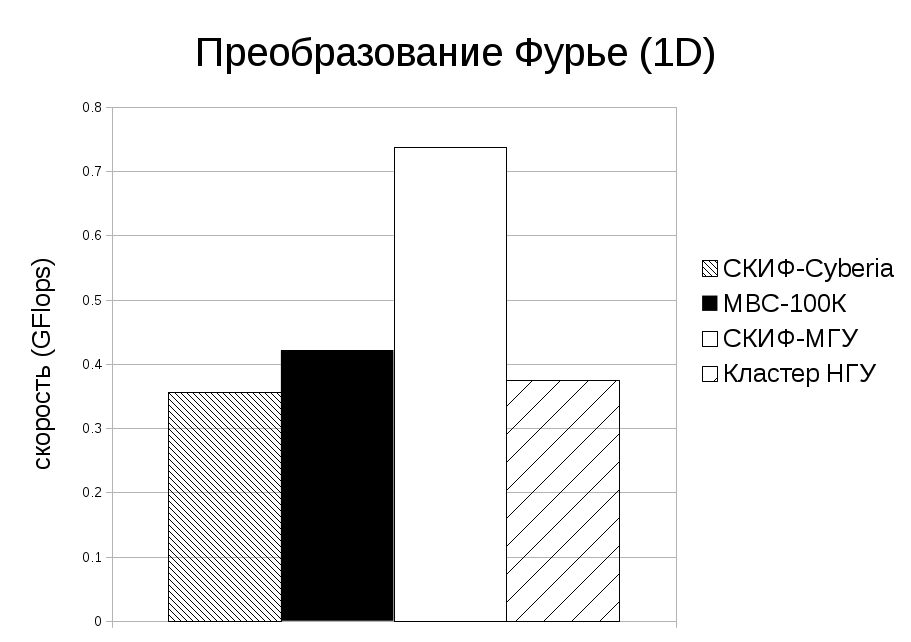
\includegraphics[height=7cm,keepaspectratio]{images/processor_FLOPS.png}
	\end{center}
	\caption{Производительность процессоров Intel Xeon, измеренная в ходе выполнения одномерного преобразования Фурье на некоторых кластерах. Размерность преобразования $N=64$. Измерения выполнены в 2010 г.}
	\label{procs_flops}
\end{figure} 

\section{О влиянии организации данных на результат измерения производительности процессоров}

Модельные частицы расположены внутри расчетной области случайным образом. Если даже модельные частицы расположены рядом в массиве, где хранятся их координаты,  то сами значения координат будут близкими только вначале. В дальнейшем модельные частицы перемешиваются. Это означает, что обращения к трехмерным массивам, содержащим электрическое и магнитное поля, являются неупорядоченными,  и использование кэш-памяти в данном случае не позволяет сократить время счета. 

Использование кэш-памяти было бы более эффективным, если бы частицы были упорядочены. Тогда значения полей, загруженных в кэш при расчете движения некоторой частицы, могли бы быть использованы и для следующей частицы, если она расположена близко. 

Для этого достаточно упорядочить частицы по ячейкам сетки, то есть, хранить каким-то образом вместе все частицы, которые расположены внутри каждой ячейки. Это означает, что полная сортировка массива частиц не нужна, так как с точки зрения использования кэш-памяти не имеет значения, как частицы расположены внутри ячейки. 

Модельные частицы, принадлежащие некоторой ячейке сетки, можно хранить в виде связанного списка или в виде массива. Преимущества списка очевидны: нет ограничения на число частиц в ячейке, простота добавления/удаления, но есть и недостатки, а именно большее по сравнению с массивом время доступа. Если же частицы каждой ячейки хранятся в виде массива (статического массива), то применительно к трехмерной задаче для двух сортов частиц это даст 5-мерный массив для одной только координаты X всех частиц (напомним, что модельная частица в данном случае характеризуется шестью признаками). 

Но основная проблема в случае статического массива - это максимальное число частиц в ячейке. Это означает, что заранее неизвестно, какой длины массив потребуется для хранения всех частиц в каждой ячейке. Из проведенных расчетов известно, что максимальное значение плотности электронов было равно 5 (в единицах начальной плотности). Таким образом, можно было бы задать длину массива частиц в каждой ячейке 5N, где N - число частиц в ячейке в начальный момент времени. Но в этом случае размер массива частиц увеличится в 5 раз, а его размер составляет 70 Гб, например, для сетки 512х64х64 и N = 150. 

Использование для этой цели динамических массивов решает проблему перерасхода памяти, но создает другую: необходимость иметь внутри программы свой эффективный менеджер динамической памяти, что, возможно, является решаемой задачей, но едва ли приведет к существенному уменьшению времени работы программы в целом. 

Поэтому был реализован компромиссный вариант: для каждого сорта частиц (в данном случае 2 сорта: электроны и ионы) в каждой ячейке в целочисленном массиве длины 5N хранить номера частиц, находящихся в данный момент в данной ячейке. Номер задает позицию частицы в больших (порядка 100 млн. элементов) вещественных массивах, в которых хранятся координаты и импульсы модельных частиц. Таким образом, при перемещении частицы из одной ячейки в другую (обязательно в соседнюю - это определяется соображениями устойчивости метода частиц) перемещается только номер частицы: он удаляется из массива номеров, описывающих текущую ячейку, и добавляется в массив номеров одной из соседних ячеек. Внутри самих массивов координат и импульсов частицы никогда не перемещаются. 

Также был реализован вариант с хранением частиц каждой ячейки в виде связанного списка. В этом случае имеется 4-мерный массив указателей, задающий первый элемент списка в каждой ячейке, и отсутствуют большие массивы: вся информация по частицам хранится только в списках. 

В обоих вариантах на вход процедуры интегрирования уравнений движения модельных частиц подаются шесть небольших (размером не более 5N) массивов, хранящих координаты и импульсф частиц для каждой конкретной ячейки. Эти массивы формируются либо на основе списка частиц, либо на основе массива номеров частиц этой ячейки. 

Таким образом, имеются следующие варианты организации частиц в программе:
\begin{enumerate}
	\item Исходный неоптимизированный вариант; 
	\item Хранение значений поля в 4-мерном массиве; 
	\item Упорядочивание частиц с помощью массивов номеров; 
	\item Упорядочивание частиц с помощью связанного списка; 
\end{enumerate}

Далее рассмотрим результаты тестов, показывающих эффективность выполненной оптимизации. Тестовые расчеты проводились на рабочей станции с процессором AMD Phenom, и на кластере Новосибирского Государственного Университета, оснащенного процессорами Intel Nehalem. В обоих случая была выбрана сетка такого размера, что даже один трехмерный массив, содержащий, например, одну из компонент поля, заведомо не помещается в кэш. 
Размер сетки: (рабочая станция, процессор Phenom, последовательный счет) 64х32х32 узла, 50 частиц в ячейке, (кластер, процессор Nehalem, в пересчете на один процессор), 512х2х64 узла, 50 частиц в ячейке. 

\begin{table}[ht]
	\begin{center}
		\caption{Время вычислений и время комуникаций в зависимости от числа  процессов, в секундах.}
		\begin{tabular}{|c|c|c|}
		 процессор                                & Phenom & Nehalem \\ \hline   	
Исходный неоптимизированный вариант               & 13.25  & 7.22    \\ \hline   	
Хранение значений поля в 4-мерном массиве         & 8.8    & 6.72    \\ \hline 
Упорядочивание частиц с помощью массивов номеров  & 12.51  & 5.67    \\ \hline 
Упорядочивание частиц с помощью связанного списка & 10.5   & 10.3    \\ \hline 
Сочетание вариантов 2 и 3			              & 10.92  & 3.67    \\ \hline 
			\hline	
\end{tabular}
\end{center}
\end{table}			



Отсюда можно сделать вывод, что сочетание упорядочивания модельных частиц и хранения значений поля в одном 4-мерном массиве приводит к значительному сокращению времени вычислений с частицами, в данном случае, почти в 2 раза. Хранение частиц в виде связанных списков оказалось неэффективным для процессора Nehalem, но, возможно, окажется полезным на других архитектурах (так позволяют думать измерения времени на процессоре Phenom)или в тех случаях, когда установить максимальное число частиц в ячейке 
невозможно. 

\section{Оценка возможности выполнения крупномасштабных трехмерных расчетов}

Проведены тестовые расчеты с целью эффективности распараллеливания и масштабируемости разработанных алгоритмов для моделирования взаимодействия электронного пучка с плазмой, а также с целью выяснения реальных возможностей суперЭВМ по проведению физических расчетов. Показано, что текущая версия программы позволяет проводить расчет на трехмерной сетке размером 3503 узлов при 100 частицах в ячейке за 1 сутки на 10 ядрах суперкомпьютера «Ломоносов», или 42 млн.узлов. Эффективность распараллеливания составила 92 % для максимального использованного числа ядер: 100 для кластера НГУ и 200 для кластера «Политехник».  Таким образом раработанная программа может считаться готовой к проведению запланированных расчетов на сетках размерностью свыше 100 млн. узлов.















Целью расчетов,  является ответ на вопрос, какие расчеты (т.е. какой размерности) могут бытть проведены на доступных суперЭВМ, на каком количестве процессоров (или процессорных ядер) и за какое время. 
Для того, чтобы получить ответ на этот вопрос, было запущено большое количество тестовых расчетов, параметры которых приведены в отчете прошлого месяца. Эти тестовые расчеты носят предварительный характер, и проводятся также с целью выяснения реальных возможностей суперЭВМ для проведения физически содержательных расчетов, выполнение которых запланировано   на июль 2017. 	Расчеты проводились на следующих суперЭВМ: кластер СпбГТУ “Политехник”, кластер НКС-1П (ССКЦ СО РАН), кластер НГУ,  суперкомпьютер НИВЦ МГУ “Ломоносов”. Первоначально запланированные расчеты на кластере НКС-30Т  (ССКЦ СО РАН) не проводились в силу того, что его архитектура идентична таковой для кластера НГУ, а также технических проблем, возникших на НКС-30Т в июне 2017.
Следует отметить, что значительная часть запущенных расчетов не была успешно завершена – как по субъективным причинам (недостатки разработанной программы), так и по объективным (заполненность очереди задач, низкая производительность коммуникационного оборудования, системные ограничения – например, на количество одновременно запущенных задач, или занятых узлов). Основные параметры успешно проведенных расчетов показаны в таблице 1. 
В ходе проведения тестовых расчетов было получено большое количество числовых характеристик – время расчета для различных сеток (таблица 1), продолжительность коммуникационных операций (рис. 2, 3), эффективность в сильном и слабом смысле (рис.3, 4), причем все это как для лагранжевой, так и для эйлеровой и декомпозиции и для четырех различных суперЭВМ. 






Однако с точки зрения проекта (с точки зрения проведения реальных физических расчетов) имеет смысл только один параметр – оценка размерности расчета продолжительностью 10 тыс. временных шагов,  который можно провести за сутки в данной параллельной конфигурации (при заданном числе процессорных ядер и заданном числе подобластей, на которые разделяется расчетная область), т.е. без увеличения времени коммуникаций. Под размерностью расчета понимается количество узлов N трехмерной кубической сетки (полный размер сетки N*N*N узлов) (одинаковое количество узлов по каждому направлению?) вдоль одного измерения, рис.1. Число частиц во всех тестовых расчетах 100 в ячейке, соответственно и при проведении оценок будем исходить из этого. Размерность расчета оценивается следующим образом:
за основу берется продолжительность временного шага, реально измеренная в ходе тестового расчета
вычисляется отношение времени 8.64 сек. (один шаг из 10 тыс., проводимых за сутки) к измеренной продолжительности временного шага, обозначим это отношение k
размер сетки, реально имеющийся в данном тестовом расчете, умножается на k, и из произведения извлекается кубический корень
в том случае, когда сетка вычисленного размера (вместе с частицами) не помещается в память узла, указывается максимально возможный по объему памяти размер (в основном это касается “Ломоносова”)
Вычисленная таким образом размерность задачи приведена в таблице 1 в выделенной колонке. Кроме того, приведены основные параметры и числовые характеристики тестовых расчетов, обозначенные следующим образом:
\begin{itemize}
\item $N_X, N_Y, N_Z$  - размер сетки по каждому из измерений
\item $P_{ALL}$  - общее количество процессорных ядер
\item $P_{SUB}$  - число подобластей
\item $T$ – длительность тестового расчета (50 временных шагов), сек.
\item $\Delta t$  - длительность временного шага, сек.
\item $T_{A} - длительность операции MPI\_Allreduce (суммирование токов по всей области), сек.
\item $T_{S}$ - длительность операции MPI_Sendrecv (обмен граничными значениями), сек.
\begin{itemize}
	


\begin{table}[ht]
\begin{center}
\caption{Время вычислений и время комуникаций в зависимости от числа  процессов.}
\begin{tabular}{|c|c|c|c|c|c|c|c|c|c|c|}
\hline			
Кластер & $N_X$ & $N_Y$ & $N_Z$ &$P_{ALL}$&$P_{SUB}$ &$T$&$\Delta$ & $T_{A} &  $T_{S}$ \\\hline
НГУ     & 100   & 100   & 20    &  1        & 1         & 39.1  & 0.78 & 0.004         & 0          \\\hline
НГУ     & 100   & 100   & 20    &  2        & 1         & 21.49 & 0.42 & 0.0029         & 0         \\\hline
НГУ     & 100   & 100   & 20    &  2        & 2         & 40.37 & 0.8 & 0.097         & 0.022       \\\hline
НГУ     & 100   & 100   & 20    &  4        & 1         & 9.9 & 0.19 & 0.0036         & 0           \\\hline
НГУ     & 100   & 100   & 20    &  4        & 2         & 16.1 & 0.32 & 0.004         & 0.0094      \\\hline
НГУ     & 100   & 100   & 20    &  10       & 1         & 6.7 & 0.13 & 0.0026         & 0      \\\hline
НГУ     & 100   & 100   & 20    &  100      & 1         & 4.0   & 0.08 & 0.0059         & 0      \\\hline
НГУ     & 500   & 500   & 20    &  20       & 1         & 714.9 & 14.2 & 6.89         & 0      \\\hline
<<Политехник>> & 100   & 100   & 20    &  4       & 2         & 13.8 & 0.27 & 0.0069         & 0.0035      \\\hline
<<Политехник>> & 100   & 100   & 20    &  100     & 10        & 2.4 & 0.048 & 0.00223        & 0.001      \\\hline
<<Политехник>> & 500   & 500   & 20    &  50       & 5        & 70.7 & 1.4 & 0.0014         & 0.006      \\\hline
<<Политехник>> & 500   & 500   & 20    &  100       & 10      & 64.0 & 1.28 & 0.054         & 0.029      \\\hline
<<Политехник>> & 500   & 500   & 20    &  200       & 20      & 70.2 & 1.4 & 0.096          & 0.009      \\\hline
<<Ломоносов>> & 100   & 100   & 20    &  10       & 1         & 2.0 & 0.04 & 0.003         & 0      \\\hline
<<Ломоносов>> & 100   & 100   & 20    &  100       & 1        & 2.5 & 0.05 & 0.005         & 0      \\\hline
НКС-1П        & 100   & 100   & 20    &  100       & 1        & 28.9 & 0.57 & 0.0075         & 0      \\\hline
НКС-1П        & 100   & 100   & 20    &  200       & 1        & 35.1 & 0.7 & 0.069         & 0      \\\hline

\end{tabular}
\end{center}
\end{table}

Рис. 2. Эффективность параллельного выполнения на кластере НКС-1П. На рисунке видно, что доля времени, расходуемого на коллективные операции незначительно уменьшается с ростом числа процессоров.


Рис. 3. Уменьшение времени счета одного временного шага с увеличением числа ядер на кластере НГУ.


Рис.4. Эффективность распараллеливания, вычисляемая как отношение времени вычислений к полному времени расчета, кластер НГУ.

Рис.5. Эффективность распараллеливания, вычисляемая как отношение времени вычислений к полному времени расчета, кластер 





\section{Расчет производительности системы памяти}
Во \textit{втором разделе} описано измерение производительности системы памяти, основанное на измерении времени расчета движения модельных частиц, при этом благодаря алгоритмически особенностям метода частиц в ячейках удается исключить использользование кэш-памяти и производить измерение скорости доступа именно к оперативной памяти.

Переход от фактически измеренной величины, времени выполнения расчета движения модельных частиц выполнялся из следующих соображений: на каждое из используемых ядер приходится 2.5 млн. модельных частиц, каждая частица занимает 48 байт, кроме того, для расчета движения частицы необходимы значения электрического и магнитного полей в той ячейке сетки, где находится частица. Это означает, что для каждой из 6 компонент электромагнитного поля загружается 8 значений, соответствующих вершинам параллелепипеда, то есть ячейки сетки. 

Более того, по результатам расчета движения модельной частицы вычисляется вклад данной частицы в ток. Для каждой из трех меняются значения в 4 узлах сетки компоненты тока, которые вместе с новыми значениями координаты и импульса модельной частицы сохраняются в оперативную память.

Таким образом для каждой модельной частицы загружается из памяти 432 байта и сохраняется 144 байта, общий поток данных составляет 576 байт на одну частицу.

\textbf{в третью главу - раздел про перенос на Phi с текстами}


\begin{figure}[htb]
	\begin{center}
		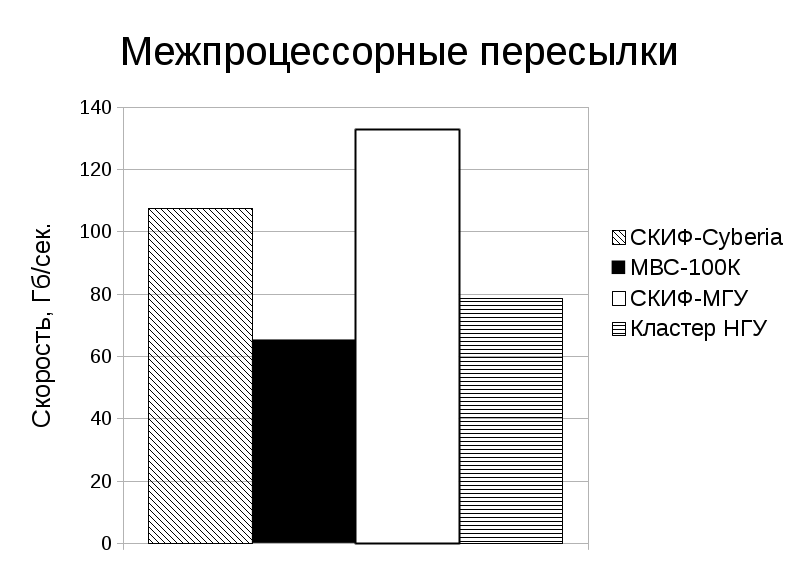
\includegraphics[height=7cm,keepaspectratio]{images/data_load_GBsec.png}
	\end{center}
	\caption{Скорость загрузки данных из оперативной памяти на этапе расчета движения модельных частиц на некоторых кластерах. Количество модельных частиц: 2.5 млн. на каждое процессорное ядро. Измерения выполнены в 2010 г.}
	\label{PIC_RAM}
\end{figure}
Следует отметить, что вопрос о сравнении чисел на рис. \ref{PIC_RAM} с техническими характеристиками шины памяти 
является второстепенным. Основной вопрос в данном случае - это измерение скорости работы памяти фактически доступной для расчетного приложения.

\subsubsection{Расчет производительности коммуникационной сети}
В \textit{третьем разделе} приведена методика измерения быстродействия коммуникационной сети на основе анализа времени работы MPI-процедур, осуществляющих обмен граничными значениями между отдельными подобластями при решении уравнений Максвелла и при пересылке модельных частиц. В силу того, что при этом используются различные виды коммуникационных функций  - как блокирующие, так и не блокирующие, как парные, так и коллективные, при использовании эйлерово-лагранжевой декомпозиции - это позволяет набрать в течение одного расчета большую базу данных для получения знаний о структуре коммуникационной сети, времени прохождения сообщений в зависимоссти от размера, системных таймаутах и пр. 

%		На  рисунке приведено скорость обмена данными между процессами (график из статьи в Мб/сек) 
%		\textbf{перерисовать графики МВС-100К и Ломоносов в общей части}	
%		
%		
%		Сравнение графиков ускорения, полученных на МВС-100К, Ломоносов НГУ и пр.

\section{Формула для комплексной оценки ВС}
\label{complex_evaluation}
В \textit{четвертом разделе} приведено обоснование формулы, на основании которой выносится оценка ВС по материалам проведенных тестов. При этом важно отметить, что оценка является не сравнительной - относительно других ВС, а абсолютной - с точки зрения математического моделирования. 

В частности, для того, чтобы параллельная ВС могла быть признана адаптированной к задачам математического моделирования, она должна соответвовать следующим требованиям:
\begin{enumerate}
	\item Относительно высокая производительность коммуникационной сети, позволяющая пересылать все необходимые для расчета данные, не задерживая вычислений
	\item Очень высокая пропускная способность дисковой подсистемы, обеспечивающая сохранение больших объемов данных, полученных в результате счета  	
\end{enumerate}

Важно отметить, что названы относительные показатели, обеспечивающие возможность пересылать и сохранять данные, без ущерба для скорости вычислений. Именно это и означает  комплексную пригодность ВС к решению задач математического моделирования, т.е. результаты счета сохраняются на диск с той же скоростью, с которой пересылаются данные между узлами данной ВС, и более того, эта скорость не намного меньше скорости вычислений.

Для того, чтобы все три упомянутые величины могли быть использованы в одной формуле, необходимо 
\begin{itemize}
	\item привести эти величины к одной размерности (скорость вычислений выражается во флопсах, скорость обмена данными - в гигабайтах в секунду)
	\item представить обобщенные коэффициенты, позволяющие сравнивать объем данных, сохраняемых на диск и объем данных, пересылаемых по коммуникационной сети ВС  
\end{itemize}


Для решения обоих этих задач использованы усредненные данные расчетов по методу частиц в ячейках на различных ВС. Данный метод может быть использован как оценка снизу, т.е. пригодность некоторой ВС для проведения расчетов по методу частиц в ячейках может трактоваться как возможность проведения расчетов по широкому спектру вычислительных методов, причем, как правило, с большей эффективностью.

Итак, коэффициент перевода из флопсов в байты в секунду для расчетов с частицами равен
$k_{f2b} = 500/576$ = 0.86   
и коээфициент для перевода объема данных, сохраняемых на диск к объему данных, пересылаемых по коммуникационной сети, аналогично, для частиц равен (усредненно):
$k_{MPI} = 0.05$ 
Это объясняется тем, что в среднем не более 5\% частиц пересылается между подобластями.
В итоге формула оценки $\xi$ имеет вид:
$$
\xi = \frac{W_{MPI}} {k_{f2b} W_{PIC}}, 
$$
при условии, что $W_{disc} \approx W_{MPI}$,
здесь $W_{disc}$ - скорость работы дисковой подсистемы (байт/сек), $W_{MPI}$
- скорость пересылки данных по сети - (байт/сек) и $W_{PIC}$ - скорость расчета по частицам (во флопсах).	

